\documentclass[conference]{IEEEtran}
\IEEEoverridecommandlockouts
% The preceding line is only needed to identify funding in the first footnote. If that is unneeded, please comment it out.

% add this package to use [H]
\usepackage{float}

\usepackage{cite}
\usepackage{amsmath,amssymb,amsfonts}
\usepackage{algorithmic}
\usepackage{graphicx}
\usepackage{textcomp}
\def\BibTeX{{\rm B\kern-.05em{\sc i\kern-.025em b}\kern-.08em
    T\kern-.1667em\lower.7ex\hbox{E}\kern-.125emX}}
\begin{document}

\title{CS 289A Final Project\\
Driving motion prediction using machine learning
}
\author{
\IEEEauthorblockN{Hengbo Ma}
\IEEEauthorblockA{\textit{SID : 3033121067} \\
hengbo\_ma@berkeley.edu}
\and
\IEEEauthorblockN{Jessica Leu}
\IEEEauthorblockA{\textit{SID : 3033088125} \\
jess.leu24@berkeley.edu}
\and
\IEEEauthorblockN{Franklin Zhao}
\IEEEauthorblockA{\textit{SID : 3033030808} \\
qingan\_zhao@berkeley.edu}
\and
\IEEEauthorblockN{Yujun Zou}
\IEEEauthorblockA{\textit{SID : 27004846} 
\\
yujun\_zou@berkeley.edu}
}

\maketitle

\section{Hidden Markov Model}
\subsection{Description}
The Hidden Markov Model (HMM) is a statistical model originally proposed by Baum et. al. \cite{hmm1}, which is used for describing a Markov process with unobserved states \cite{hmm2}. The most crucial part when applying this model is to identify those hidden states from the observed states, so that such states can be used for further analysis, like pattern recognition. 

In normal Markov Models, all states are visible to the observer, so that the only parameters should be transition probabilities. However, in HMM, the states are not directly visible, while the variables (or let us say, outputs) that dependent on those states are visible. Each of the state has a probability distribution over those outputs. Hence, the state can be analyzed and identified using the outputs from which some information in the hidden states can be provided.

\subsection{Principles and methodologies}
HMM can be regarded as a generalized form of the Urn problem with replacement \cite{hmm3}. For example, in this project, assume that we only have two categories of hidden states (0/1), where ``0" represents the current vehicle take the lead in a 2-vehicle group, while ``1” represents the other way around. The state in each time step correspond to a trajectory described in the features that extracted from the labeled data mentioned previously. For class 0, the probability of the trajectory $tr_1$ is $P_{0(tr_1)}$; Similarly, class 1 would be $P_{1(tr_1)}$ for the trajectory $tr_1$. Now, considering a time series, we do not know which vehicle take the lead in each step, but all trajectories are given (as training and test data). If we extract 10 time steps from data, we would get 10 values in the range of all possible trajectories, such as  $tr_1, tr_2, tr_3, tr_4, tr_5, tr_6, tr_7, tr_8, tr_9, tr_{10}$. These 10 values extracted from the data are called visible states, or ``outputs" as mentioned earlier. For HMM in our project, the hidden states are basically the series of the leading status in these 10 steps (i.e., 0/1). In this scenario, HMM can be visualized as shown in Figure~\ref{fig:HMMcar}.
\begin{figure}[H]
	\centering
	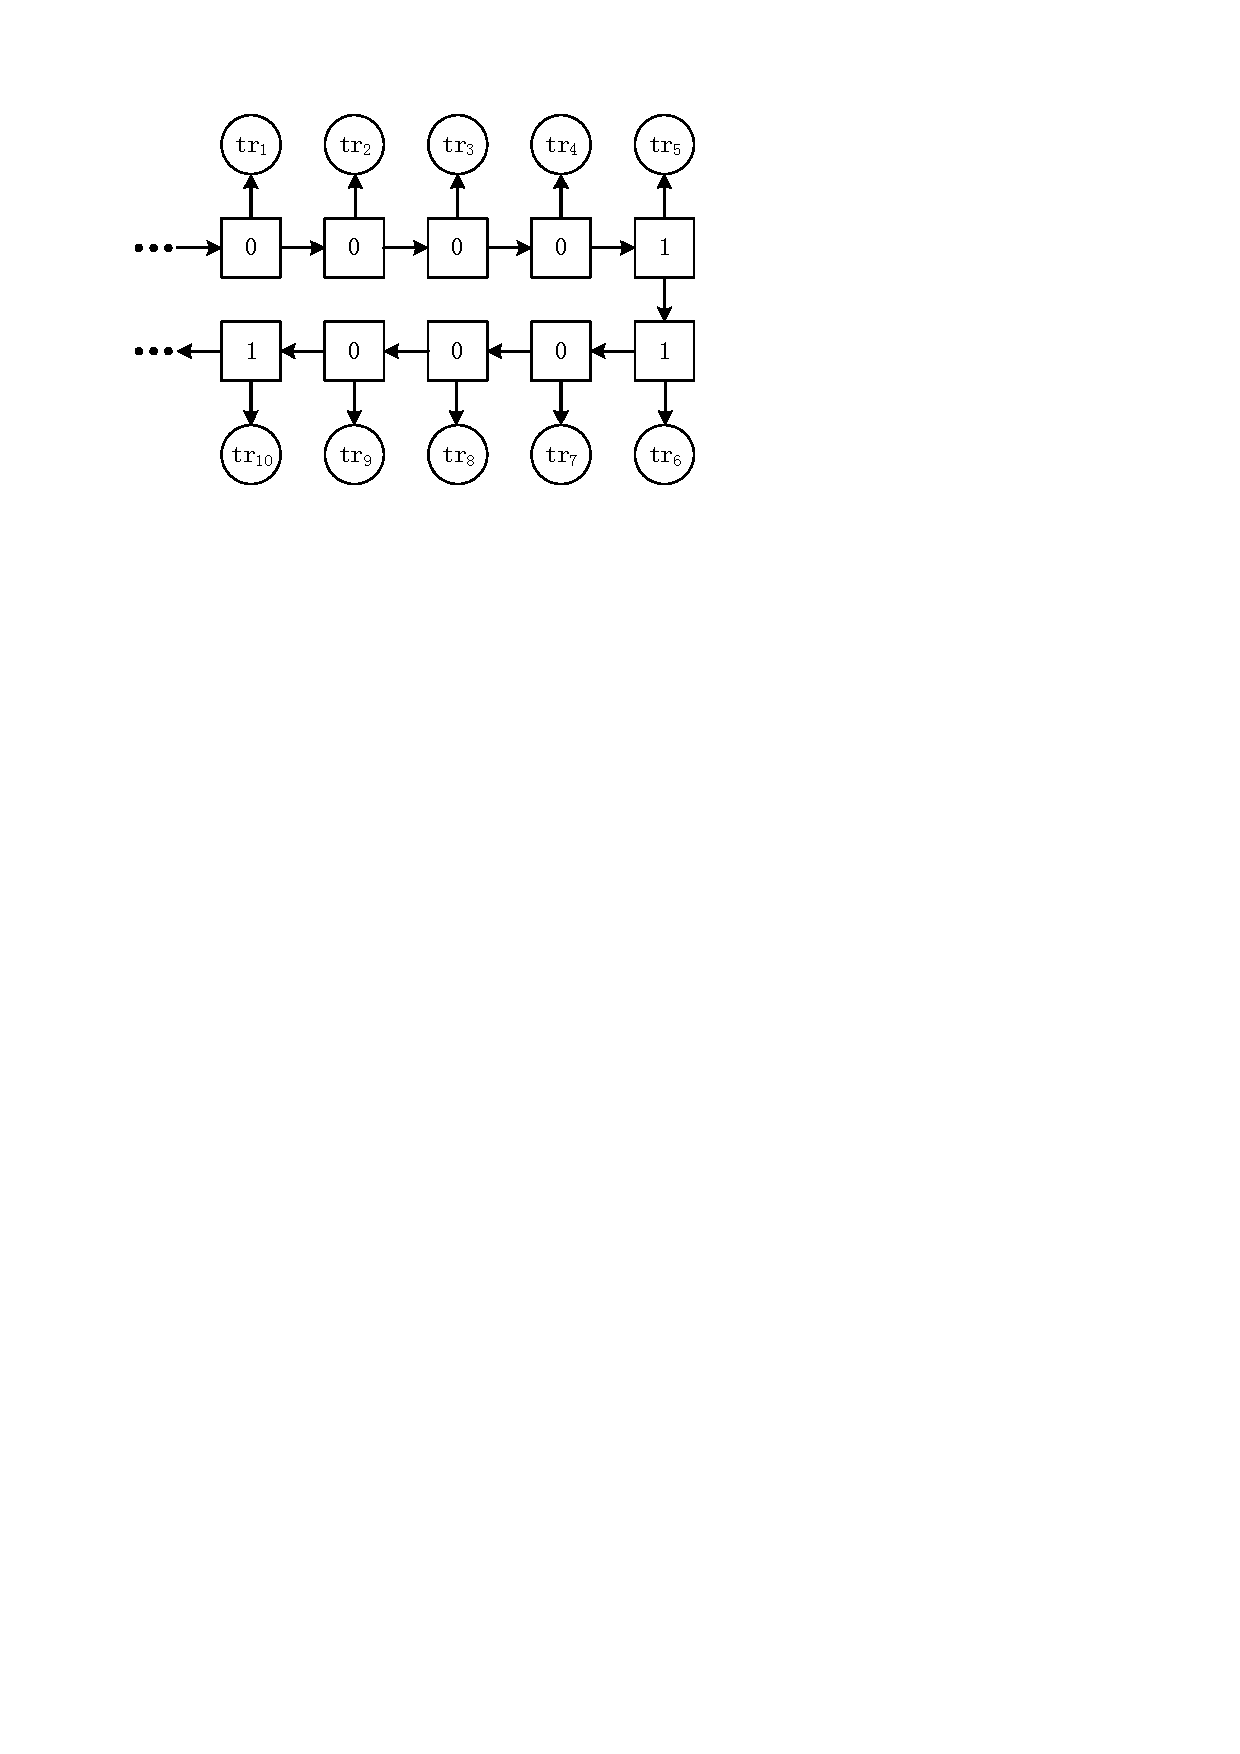
\includegraphics[scale=0.9]{HMMcar.pdf}
	\caption{HMM in a 2-vehicle group}
	\label{fig:HMMcar}
\end{figure}

The reason those leading status are the hidden states is that there is a transition probability between the two classes of states (0/1). In this example, the probability of the next state after class 0 is $P_{00}$ for class 0, $P_{01}$ for class 1, Similar for the state after class 1. In real-word HMM problems, those probabilities does not have to be the same and can be assigned to any possible values, as shown in Figure~\ref{fig:trasitionCar}. 
\begin{figure}[H]
	\centering
	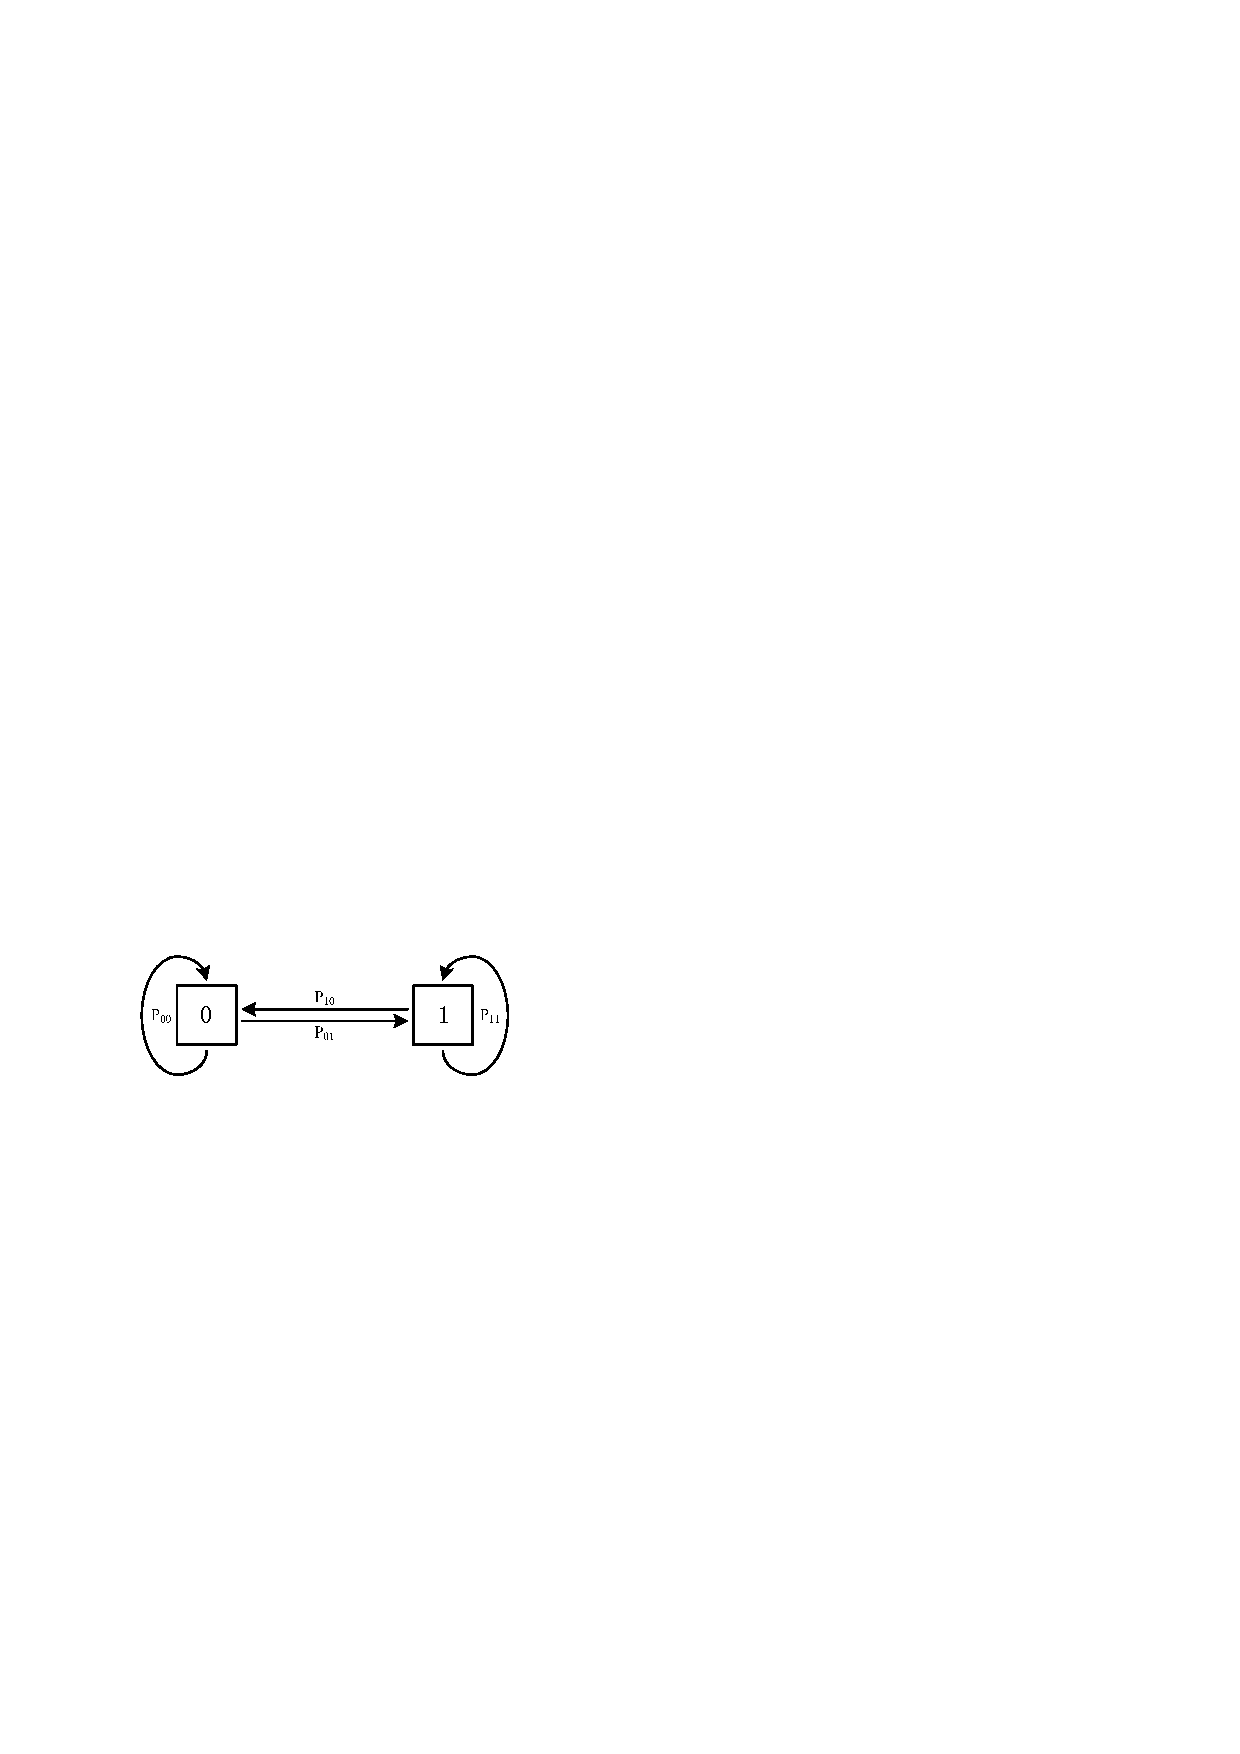
\includegraphics{transitionCar.pdf}
	\caption{Transistion probabilities in HMM}
	\label{fig:trasitionCar}
\end{figure}

Figure~\ref{fig:HMMmodel} illustrates the states change in a HMM. Denote the state in time $t$ as $q(t)$, observation as $o(t)$. From those arrows we know that $q(t)$ is related to $q(t-1)$; $q(t-1)$ is related to $q(t-2)$, and so forth, while $o(t)$ is only related to the corresponding $q(t)$. It is obvious that in this architecture, $q(t)$ is the hidden state and $o(t)$ is the output. If there are $N$ possible values for $x(t)$, then $x(t+1)$ would be $N$ possible values as well (2 in our case). Hence, there are $N^2$ possibilities from $t$ to $(t+1)$. If there are $M$ possible values for the observed $o(t)$, then the model complexity for $q(t)$ to $o(t)$ is $O(MN)$. If $o(t)$ is a vector in $M$ dimensions, then the complexity would be $O(M^2N)$.
\begin{figure}[H]
	\centering
	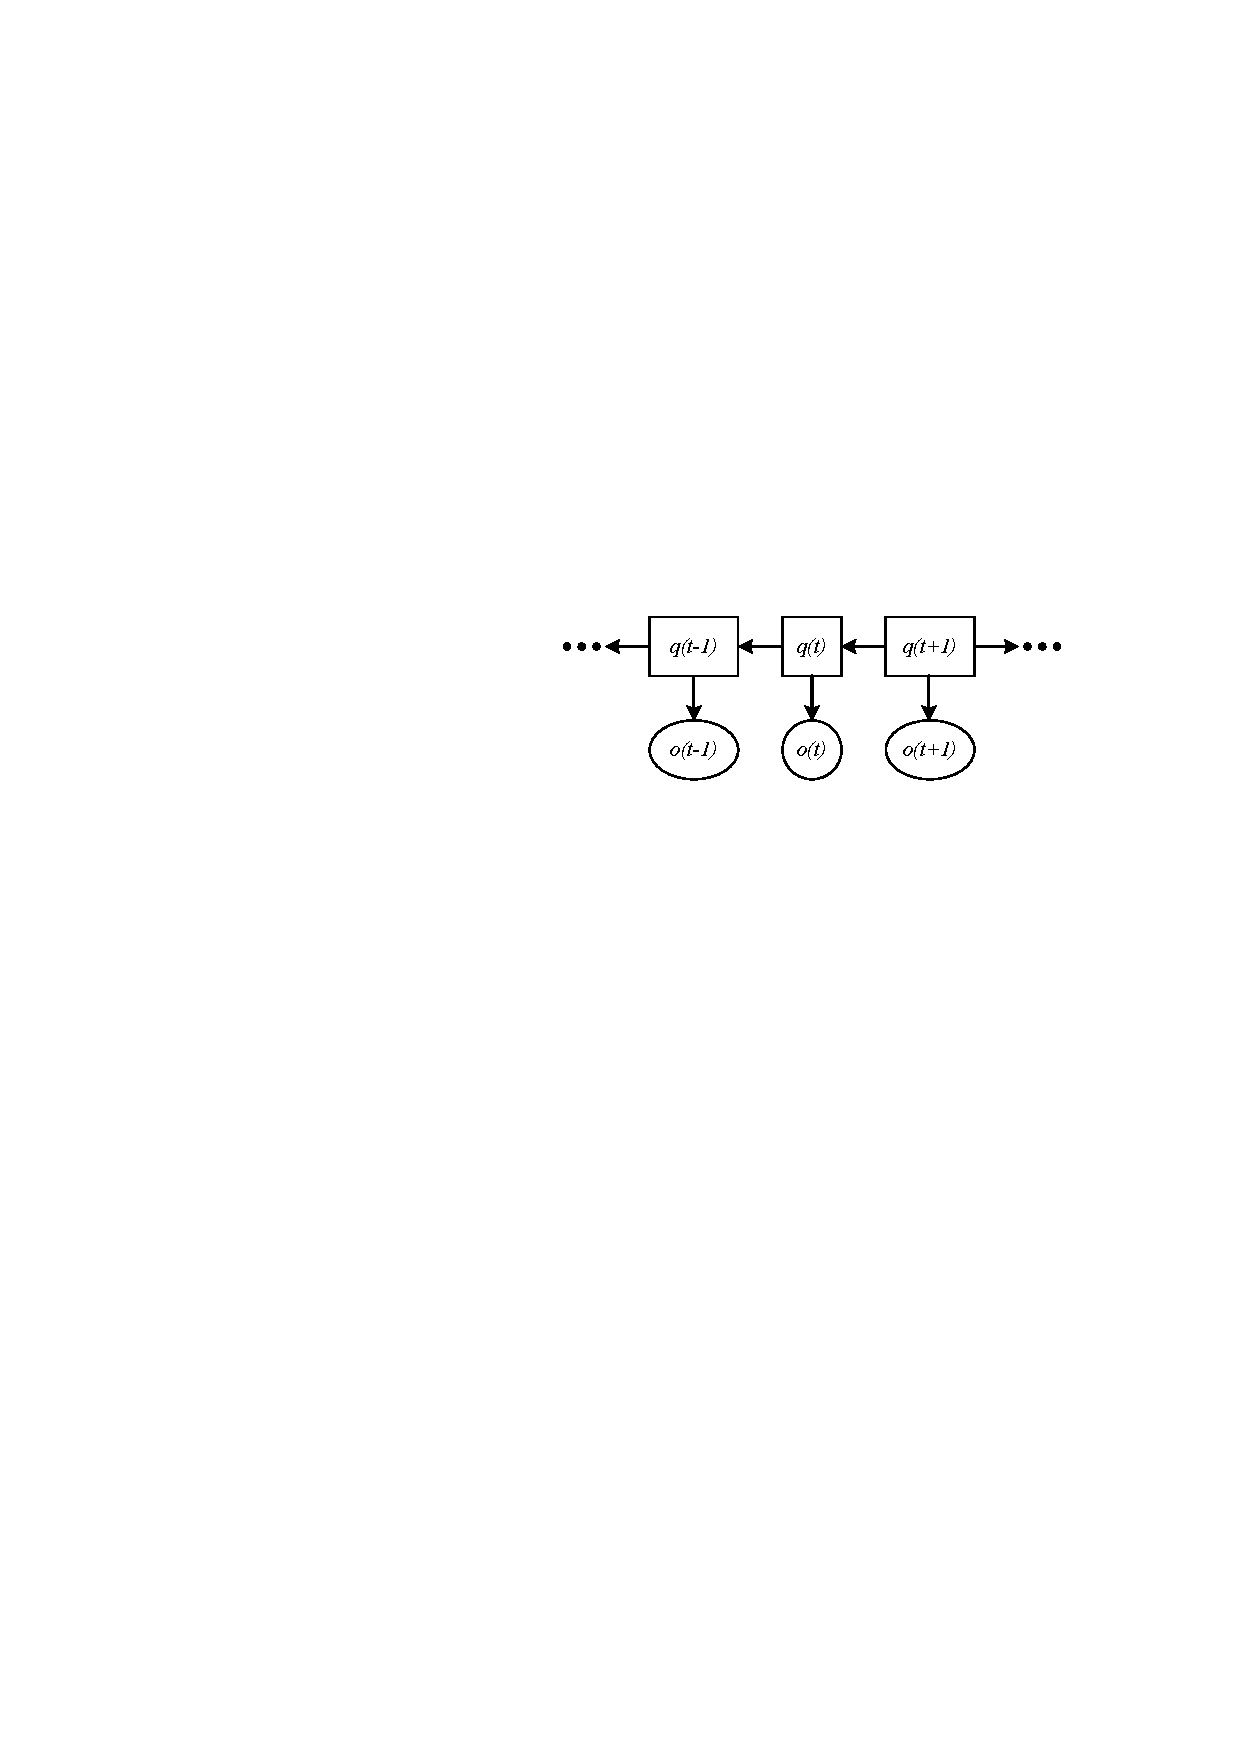
\includegraphics{HMMmodel.pdf}
	\caption{Architecture of an instatiated HMM}
	\label{fig:HMMmodel}
\end{figure}

Given a HMM length $m$, denote the output as $O=\{o_1, o_2,\dots o_m\}$; hidden state as $Q=\{q_1, q_2,\dots q_m\}$. The probability model of an HMM can be described as:
\begin{equation}
P(o)=\sum_{Q}P(o|q)P(q)
\end{equation}

\subsection{HMM learning using EM}
First denote the HMM parameters as $\lambda$ that contains 5 elements $(S,V,A,B,\pi)$, where $S$ represents the state set and $q(t)\in S$ ($S=\{0,1\}$ in our case); $V$ represents the output set and $o(t)\in V\ (t\in[1,T])$; $B=b_j(k)$ represents the probability distribution of the output ($b_j(k)=P(v_k|j),k\in[1,M],j\in[1,N]$); $\pi$ represents the initial probability distribution.

Generally there are 3 basic problems for HMM\cite{hmm4}: Given parameters $(S,V,A,B,\pi)$ and the output sequence $O=(o_1,o_2,\dots,o_T)$, compute the likelihood of the observations, namely $P(O|\lambda)$, which is an evaluation problem; Given parameters and the output sequence, find the most likely state sequence $Q=\{q_1, q_2,\dots q_m\}$ that produce the observations, which is a decoding problem; Given the output sequence, find the parameters $\lambda$ to maximize $P(O|\lambda)$, which is exactly the problem of our project -- learning problem. Expectation-maximization algorithm (EM) is applied to solve this kind of learning problem.

The expectation of our state variables is the probability that the state of a random variable $X$ is $i$ at time step $t$, namely $q(t)=i$. To calculate this probability, the forward variables $\alpha$, and backward variables $\beta$ are introduced.
\begin{equation}
\alpha_t(i)=P(o(1),o(2),\dots,o(t),q_t=i|\lambda)
\end{equation}
Namely, forward variables are the probability that the observations are $o(1),o(2),\dots,o(t)$ in state $i$ given $\lambda$ and time step $t$. Then the following equations can be derived:
\begin{equation}
\alpha_1(i)=\pi_ib_i(o_1),\ 1\leq i\leq N
\end{equation}
\begin{equation}
\alpha_{t+1}(j)=(\sum_{i=1}^N\alpha_t(i)a_{ij})b_jo_{t+1}, \ 1\leq t\leq T-1,\ 1\leq j\leq N
\end{equation}
\begin{equation}
P(O|\lambda)=\sum_{i=1}^N\alpha_T(i)
\end{equation}
Similarly, for backward variables we have:
\begin{equation}
\beta_t(i)=P(o(t+1),o(t+2),\dots,o(T),q_t=i|\lambda)
\end{equation}
\begin{equation}
\beta_T(i)=1,\ 1\leq i\leq N
\end{equation}
\begin{equation}
\beta_t(i)=\sum_{j=1}^Na_{ij}b_j(o_{t+1})\beta_{t+1}(j),\ 1\leq t\leq T-1,\ 1\leq i\leq N
\end{equation}
\begin{equation}
P(O|\lambda)=\sum_{i=1}^N\pi_ib_i(o_1)\beta_1(i)
\end{equation}
``E" step:

Denote the probability that the state is $i$ in time step $t$ and $j$ in time step $t+1$ given the parameters $\lambda$ and the observation sequence $O$ by $\xi_t(i,j)$. Then the following equation can be derived:
\begin{equation}
\begin{array}{rl}
\xi_t(i,j)=&P(q_t=i,q_{t+1}=j|O,\lambda)\\
=&\frac{P(q_t=i,q_{t+1}=j,O|\lambda)}{P(O|\lambda)}\\
=&\frac{\alpha_t(i)a_{ij}b_j(o_{t+1})\beta_{t+1}(j)}{P(O|\lambda)}\\
=&\frac{\alpha_t(i)a_{ij}b_j(o_{t+1})(j)}{\sum_{i=1}^N\sum_{j=1}^N\alpha_t(i)a_{ij}b_j(o_{t+1})\beta_{t+1}(j)}
\end{array}
\end{equation}
Denote the probability that the state is $i$ in time step $t$ given $\lambda$ and $O$ by $\gamma_T(i)$. Then the following equation can be derived:
\begin{equation}
\gamma_t(i)=\sum_{i=1}^N\xi_t(i,j),\ 1\leq t\leq T
\end{equation}
Plugging $t$ into these equations, the expectations of the times that state $i$ changed and the times that state $i$ turned to $j$ can be obtained.\\

\noindent ``M" step:

Denote the expectation of the frequency that $i$ is the initial state by $\bar{\pi}_i$, and we have:
\begin{equation}
\bar{\pi}_i=\gamma_1(i)
\end{equation}
Similarly, denote the expectation of the times that state $i$ turned to state $j$ devided by the expectation of the times that state $i$ changed by $\bar{a}_{ij}$, and we have:
\begin{equation}
\bar{a}_{ij}=\frac{\sum_{t=1}^{T-1}\xi_t(i,j)}{\sum_{t=1}^{T-1}\gamma_t(i)}
\end{equation}
where $\bar{b}_j(k)$ is the expectation of the times that output is $k$ in state $j$ divided by the expectation of the times that any other states turned into state $j$.
\begin{equation}
\bar{b}_j(k)=\frac{\sum_{t=1}^T\gamma_t(i)\delta(o_t,v_k)}{\sum_{t=1}^T\gamma_t(i)}
\end{equation}
\begin{equation}
\delta(o_t,v_k)=\left \{ 
\begin{array}{ll}
1&\text{for }o_t=v_k\\
0&\text{otherwise}
\end{array}
\right.
\end{equation}
Hence, parameters $\lambda=(A,B,\pi)$ will be updated, and the forward and backward variables can be computed again in each iteration. The loop will keep running until the ``new" and ``old" parameters are close enough.\\

In this project, we implemented this algorithm and trained data using a Python package \textit{hmmlearn} \cite{hmm5}. 


\begin{thebibliography}{00}
\bibitem{hmm1}Baum, Leonard E., and Ted Petrie. ``Statistical inference for probabilistic functions of finite state Markov chains." \textit{The annals of mathematical statistics} 37.6 (1966): 1554-1563.

\bibitem{hmm2}Wikipedia, ``Hidden Markov model",\\ \textit{https://en.wikipedia.org/wiki/Hidden\_Markov\_model} - Access date: Apr 30, 2018.

\bibitem{hmm3}Rabiner, Lawrence R. ``A tutorial on hidden Markov models and selected applications in speech recognition." \textit{Proceedings of the IEEE} 77.2 (1989): 257-286.

\bibitem{hmm4}McCallum, Andrew, Dayne Freitag, and Fernando CN Pereira. ``Maximum Entropy Markov Models for Information Extraction and Segmentation." \textit{Icml}. Vol. 17. No. 2000. 2000.

\bibitem{hmm5}Github, ``hmmlearn”, \textit{https://github.com/hmmlearn/hmmlearn} - Access date: Apr 30, 2018.

\end{thebibliography}

\end{document}
